\documentclass[a4paper]{report}

%====================== PACKAGES ======================

\usepackage[french]{babel}
\usepackage[utf8x]{inputenc}
%pour gérer les positionnement d'images
\usepackage{float}
\usepackage{amsmath}
\usepackage{graphicx}
\usepackage{url}
%pour les informations sur un document compilé en PDF et les liens externes / internes
\usepackage{hyperref}
%pour la mise en page des tableaux
\usepackage{array}
\usepackage{tabularx}
%pour utiliser \floatbarrier
%\usepackage{placeins}
%\usepackage{floatrow}
%espacement entre les lignes
\usepackage{setspace}
%modifier la mise en page de l'abstract
\usepackage{abstract}
%police et mise en page (marges) du document
\usepackage[T1]{fontenc}
\usepackage[top=2cm, bottom=2cm, left=2.5cm, right=2.5cm]{geometry}
%Pour les galerie d'images
\usepackage{subfig}
\usepackage{titlesec}

%====================== INFORMATION ET REGLES ======================

\hypersetup{							% Information sur le document
pdfauthor = {PALARD Nicolas}
pdftitle = {Stage Master 2 Informatique -
			RealityTech},			% Titre du document
pdfsubject = {Mémoire de Projet},		% Sujet
pdfkeywords = {Research, Augmented Reality, High performance},	% Mots-clefs
pdfstartview={FitH}}					% ajuste la page à la largueur de l'écran
%======================== DEBUT DU DOCUMENT ========================

\begin{document}

%régler l'espacement entre les lignes
\newcommand{\HRule}{\rule{\linewidth}{0.5mm}}

%page de garde
\begin{titlepage}
\begin{center}

% Upper part of the page. The '~' is needed because only works if a paragraph has started.

\includegraphics[width=0.35\textwidth]{./logos/ubx}~\\[1cm]

\textsc{\LARGE Université de Bordeaux - Reality Tech}\\[1.5cm]

\textsc{\Large }\\[0.5cm]

% Title
\HRule \\[0.4cm]

{\huge \bfseries Mémoire de stage\\
				Master 2 Informatique\\
				Image et son\\}

\HRule \\[1.5cm]

% Author and supervisor
\begin{minipage}{0.4\textwidth}
\begin{flushleft} \large
\emph{Auteur:}\\
Nicolas \textsc{PALARD}\\
\end{flushleft}
\end{minipage}
\begin{minipage}{0.4\textwidth}
\begin{flushright} \large
\emph{Client:} \\
Jérémy \textsc{Laviole}\\
\emph{Référent:} \\
Vincent \textsc{LEPETIT}
\end{flushright}
\end{minipage}

\vfill


\includegraphics[width=0.22\textwidth]{./logos/logo-rt-notext}~\\[1cm]
% Bottom of the page
{\large \today}

\end{center}
\end{titlepage}

%page blanche
\newpage
~
%ne pas numéroter cette page
\thispagestyle{empty}
\newpage

\renewcommand{\abstractnamefont}{\normalfont\Large\bfseries}
%\renewcommand{\abstracttextfont}{\normalfont\Huge}

\begin{abstract}
\hskip7mm

\begin{spacing}{1.3}

Dans le cadre de mon stage de fin d'étude, j'ai eu l'occasion de travailler chez \texttt{RealityTech}, une jeune startup dans le domaine de la réalité augmentée spatiale. Durant le temps que j'y ai passé, il m'a été demandé d'étudier les objectifs, les intérêts et les apports de cette technologie. J'ai tout d'abord pu l'apprivoiser par le biais de \texttt{PapARt}, le système de projection interactif que développe la société, avec lequel j'ai développé mes premières applications. Tout au long de ces développements, j'ai découvert les enjeux mais aussi les difficultés inhérentes à de tels systèmes. Ces diverses difficultés ainsi que la rigidité de \texttt{PapARt} m'ont amené à développer un prototype d'une nouvelle plateforme pour la société, dont le but était d'offrir de meilleures performances et d'être plus robuste que le système actuel, tout en en conservant les fonctionnalités. De l'optimisation matérielle à la refonte complète de l'architecture, en passant par l'optimisation algorithmique, il m'a été demandé d'opérer sur tous les fronts afin de créer un prototype viable. Un prototype n'allant pas sans tests, j'ai du m'atteler à réaliser une batterie de tests de performance qui ont permis de mettre en lumière les avancées mais aussi les défauts de ce dernier. Les performances n'étant pas le seul critère de validation du prototype, j'ai poursuivi mon stage en développant un module Unity permettant de le mettre à profit. En plus de permettre l'évaluation de l'utilisabilité du prototype, le module devait aussi fournir aux utilisateurs développeurs de \texttt{RealityTech} la possibilité de créer des applications de réalité augmentée spatiale en résolvant, pour ces derniers, les nombreuses problématiques liées au domaine. Ainsi, pour terminer mon stage, j'ai endossé le costume de l'utilisateur développeur et ai réalisé une application de démonstration en utilisant le module nouvellement créé afin d'en réaliser l'évaluation.\\

\textit{Mot-clés:} Réalité augmentée, réalité augmentée spatiale, interface tangible, programmation haute performance, microservices, unity, processing, vision par ordinateur.

\end{spacing}
\end{abstract}


\tableofcontents
\thispagestyle{empty}
\setcounter{page}{0}
%ne pas numéroter le sommaire

\newpage

%espacement entre les lignes d'un tableau
\renewcommand{\arraystretch}{1.5}

%removing Chapter name and number
\titleformat{\chapter}[display]
  {\normalfont\bfseries}{}{0pt}{\Huge}

%====================== INCLUSION DES PARTIES ======================

~
\thispagestyle{empty}
%recommencer la numérotation des pages à "1"
\setcounter{page}{0}
\newpage

\chapter{Introduction}

Ce mémoire retracera les missions réalisées durant mon stage de Master 2 Informatique pour l'Image et le Son à l'Université de Bordeaux 1 effectué entre Avril et Septembre 2018 (6 mois) dans la société RealityTech. Ce rapport ne couvrira cependant que les 5 premiers mois du stage car la date de rendu de ce dernier précède d'un moi la date de fin du stage.

Le stage a donc été effectué chez RealityTech une jeune start-up de réalité augmentée spatiale. Issue de l'Inria de Bordeaux, l'institut national de la recherche en information et en automatique, cette dernière est la continuité d'un projet de recherche mené par Jérémy Laviole, ex ingénieur de recherche à l'Inria. PapARt\footnote{https://project.inria.fr/papart/fr/}. Paper Augmented Reality ToolKit est un kit de développement (SDK) permettant de créer des expériences de réalité augmentée sous forme d'applications de projection interactive dans des feuilles de papier. Les travaux actuellement effectués a RealityTech visent à améliorer et étendre ce système de projection. Le but est de pouvoir créer, via ce que propose la société, des expériences collaboratives où les objets physiques se mêlent parfaitement au monde numérique que ce soit en créant des interactions avec ceux ci, ou en leur rajoutant du contexte.

Actuellement, RealityTech se développe dans un incubateur de start-up appelé \texttt{La Banquiz}\footnote{http://labanquiz.com} situé 4 rue Eugène et Marc Dulout, a Pessac Centre. L'objectif de La Banquiz est de promouvoir des start-up Open Source\footnote{https://fr.wikipedia.org/wiki/Open\_source} et innovantes en leur apportant des formations, du coaching individuel et collectif, de l'aide pour la recherche de financement et tout ce qui gravite autour de l'accompagnement de jeunes entreprises.

A ce jour RealityTech ne travail qu'avec des laboratoire de recherche (comme ...) et cherche a étendre son secteur d'activité. Les systèmes proposés par la société fournissent les résultats espérés et la dynamique de celle ci s'oriente donc vers une commercialisation du produit. %Parler du fort besoin d'innovation logiciel (plateform haute performance, haut de gamme moyen de gamme bas de game. Expliquer le besoin de démo, de prototype, le salon qu'on a effecuté etc...
% Biblio : PapARt, Inria, Reality Tech, Realité Augmentée Spatiale

\section{Cadre et contexte}
\label{sec:contexte}
RealityTech fait actuellement partie de La Banquizz, un incubateur de startup situé a Pessac Centre.
% Expliquer le cadre de travail, incubateur, beaucoup de réunion, de démarchage, besoin d'applications de démonstration, besoin de prototype pour avoir des fonds etc autonomie très importante ..
% Parler du contexte  en terme de logiciel : volonté d'évolué et de partir vers une nouvelle base moins contraignante que celle présente actuellement + volonté d'ouverture au grand public (ce qui a fait que j'ai du dev unity) + modularité
% Peut être parler plus en détail de PapARt (calibration camera projecteur, expliqué qu'on travail avec des caméra, a l'échelle dans le monde réel (beaucoup de problèmes de calibration etc ...)

\begin{center}
Problématique du sujet
\end{center}


\section{Objectifs}
Le déroulement du stage a été fortement guidé par les besoins de la société.
\paragraph{Applications de démonstration}Le premier gros objectif du stage était le développement d'applications de démonstration en utilisant le produit de l'entreprise. Le but était de comprendre l'essence, le fonctionnement global du produit et ce qu'il était possible/impossible de réaliser avec celui ci. Cet objectif m'a permis d'acquérir à la fois une vision globale de l'architecture logiciel et du fonctionnement interne du kit de développement, et de l'architecture matérielle nécessaire a l'utilisation du kit. En développant ces applications de démonstration, j'ai acquis une vision globale du projet qui m'a permis d'avoir une certaine autonomie assez rapidement

\paragraph{Plateforme haute performance} Le deuxième objectif était de réaliser une preuve de concept haute performance du produit. En effet, comme je l'ai expliqué dans la partie sur le contexte (voir ~\ref{sec:contexte}), l'entreprise se lançait dans le développement d'une nouvelle plateforme haute performance.
% TODO pas fini

\paragraph{Kit de développement} Le dernière objectif était le développement d'un nouveau kit de développement pour Unity3D.  % TODO expliciter

\newpage
\chapter{Notions}
\label{chap:notions}

Le domaine d'activité qui entoure ce stage est très riche en termes de notions et de vocabulaire. Afin de mieux comprendre de quoi il va être question tout au long de ce rapport, il est nécessaire d'en définir les notions de base.

\paragraph{Réalité virtuelle}
La réalité virtuelle plus communément appelé \emph{Virtual Reality (VR)} désigne l'ensemble des environnements purement numériques (fig~\ref{fig:realityspectrum}), qu'ils soient réalistes ou non, dans lesquels aucune interaction avec l'environnement réel n'est possible et inversement. Cette réalité se base très généralement sur un casque \emph{Head Mounted Display (HMD)} dont l'utilisateur doit se munir afin d'être immergé dans un monde numérique avec lequel il peut interagir. Dans la réalité virtuelle, l'immersion est une notion importe lorsqu'il s'agit de la différenciée d'un simple programme informatique.

\begin{figure}[H]
\centering
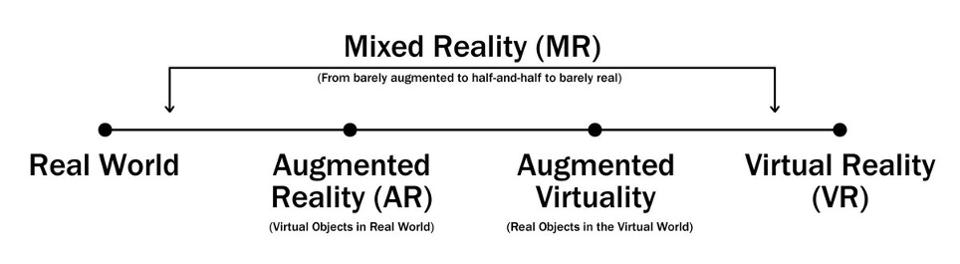
\includegraphics[width=\linewidth]{images/RealitySpectrum}
\caption{Représentation de continuum de la virtualité par Milgram et Kishino, 1995\cite{milgram1995augmented}}
\label{fig:realityspectrum}
\end{figure}

\paragraph{Réalité augmentée}
La réalité augmentée plus communément appelé \emph{Augmented Reality (AR)} quant a elle est un sous domaine de la réalité virtuelle. L'idée de la réalité augmentée est de venir superposer à l'environnement réel des éléments virtuels. Ces éléments vont alors venir "augmenter" notre monde en apportant le plus souvent des compléments d'informations. Elle est donc qualifié de sous domaine de la réalité virtuelle car l'utilisateur n'est plus immergé dans un environnement complètement numérique mais du contenu virtuel est ajouté en contexte à la vision réelle. Par abus de langage le terme de réalité augmentée est souvent utilisé pour parler de réalité mixte dont la notion est détaillé dans cette partie.
Il faut noter que ce type de réalité ne se base pas uniquement sur des \emph{HMD} mais peut être aussi apprécié à l'aide d'un téléphone par exemple (fig~\ref{fig:AR}).

\begin{figure}[H]
\centering
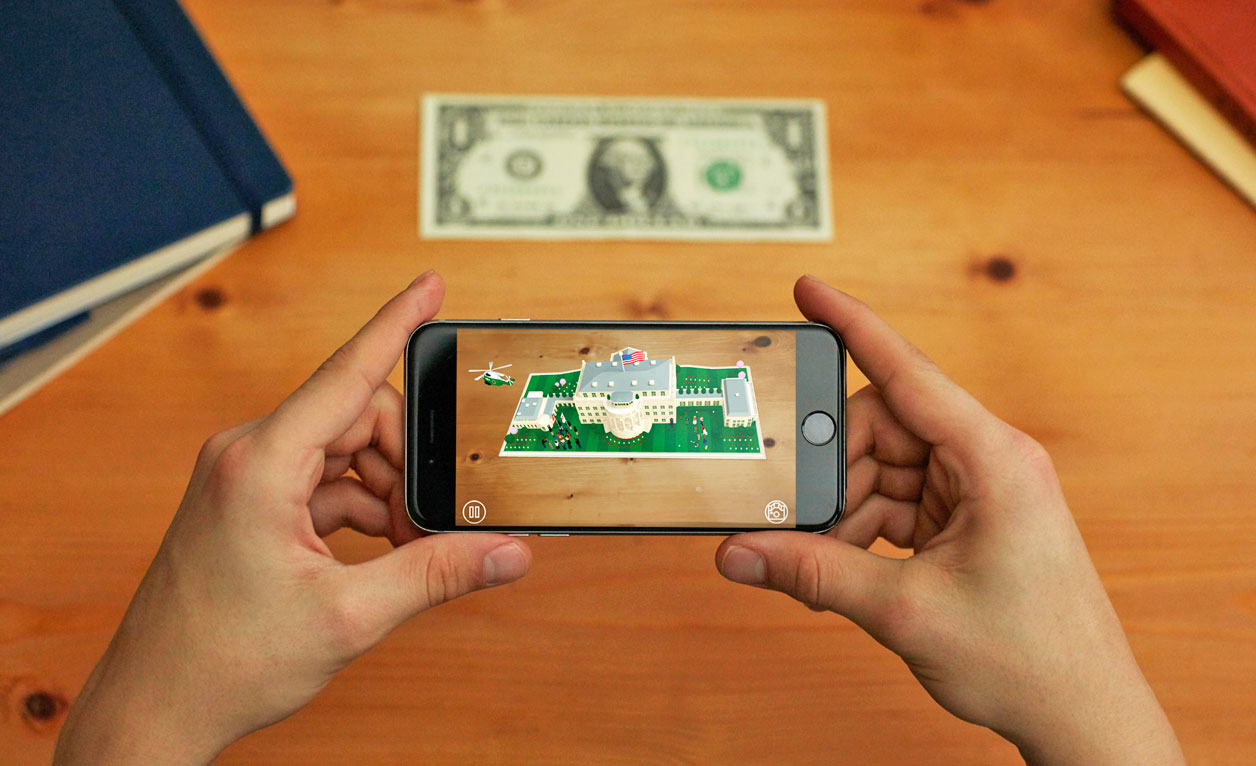
\includegraphics[width=0.55\textwidth]{images/AR}
\caption{Réalité augmentée vu au travers d'un téléphone\protect\footnotemark}\label{fig:AR}
\end{figure}
\footnotetext{Source: \href{https://www.engadget.com}{https://www.engadget.com}}

\paragraph{Réalité mixte}
La réalité mixte, ou hybride, plus communément appelé \emph{Mixed Reality (MR)}, ou \emph{Crossed Reality (XR)}, est la fusion parfaite de l'environnement numérique et de l'environnement physique (fig~\ref{fig:realityspectrum}). Dans ce "nouvel" environnement, les objets physiques et numériques coexistent et peuvent interagir entre eux et par exemple une table peut devenir une plateforme pour un personnage virtuel (fig~\ref{fig:youngconker}). Souvent confondu avec la réalité augmentée, cette dernière se différencie car elle ne propose pas seulement une visualisation des objets numériques, elle propose aussi des méthodes d'interactions avec ce contenu et c'est cette notion d'interaction qui permet de la différencier. A l'heure actuelle la réalité mixte nécessite un dispositif de type \emph{HMD} pour être appréciée comme par exemple  l'\texttt{HoloLens} de \texttt{Microsoft}.

\begin{figure}[H]
\centering
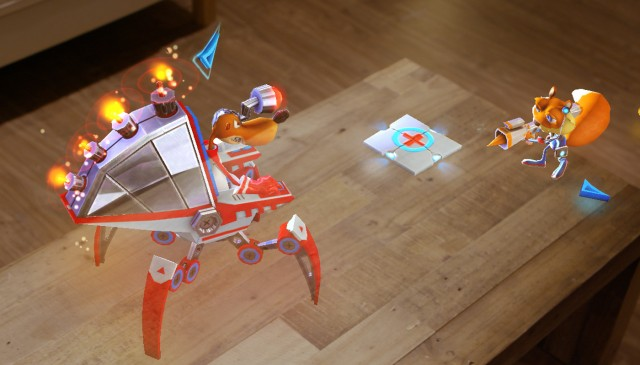
\includegraphics[scale=0.4]{images/youngconker}
\caption{Asobo Studio\texttrademark - Young Conker\copyright}
\label{fig:youngconker}
\end{figure}

\paragraph{Réalité augmentée vue au travers}
% Trouver qui l'a inventé et quand
La réalité augmentée vue au travers, plus communément appelé \emph{See Through Augmented Reality (STAR)} est une technique de visualisation de la réalité augmentée ou les éléments numériques sont vu au travers d'un écran (fig~\ref{sub:STARGO}) ou d'un \emph{HMD} (fig~\ref{sub:STARHolo}). C'est le type de visualisation le plus  utilisé actuellement. L'un des défauts majeur de ce type de visualisation est que la plus part du temps, chaque utilisateur a besoin de son propre écran ou casque pour pouvoir en profiter pleinement ce qui limite grandement les expériences collaboratives. Aussi les principaux défauts liés aux écrans s'appliquent aussi, a savoir fatigue visuel etc.  

\begin{figure}[H]
    \centering
	\subfloat[Pokémon GO - Vue au travers téléphone\protect\footnotemark]{
      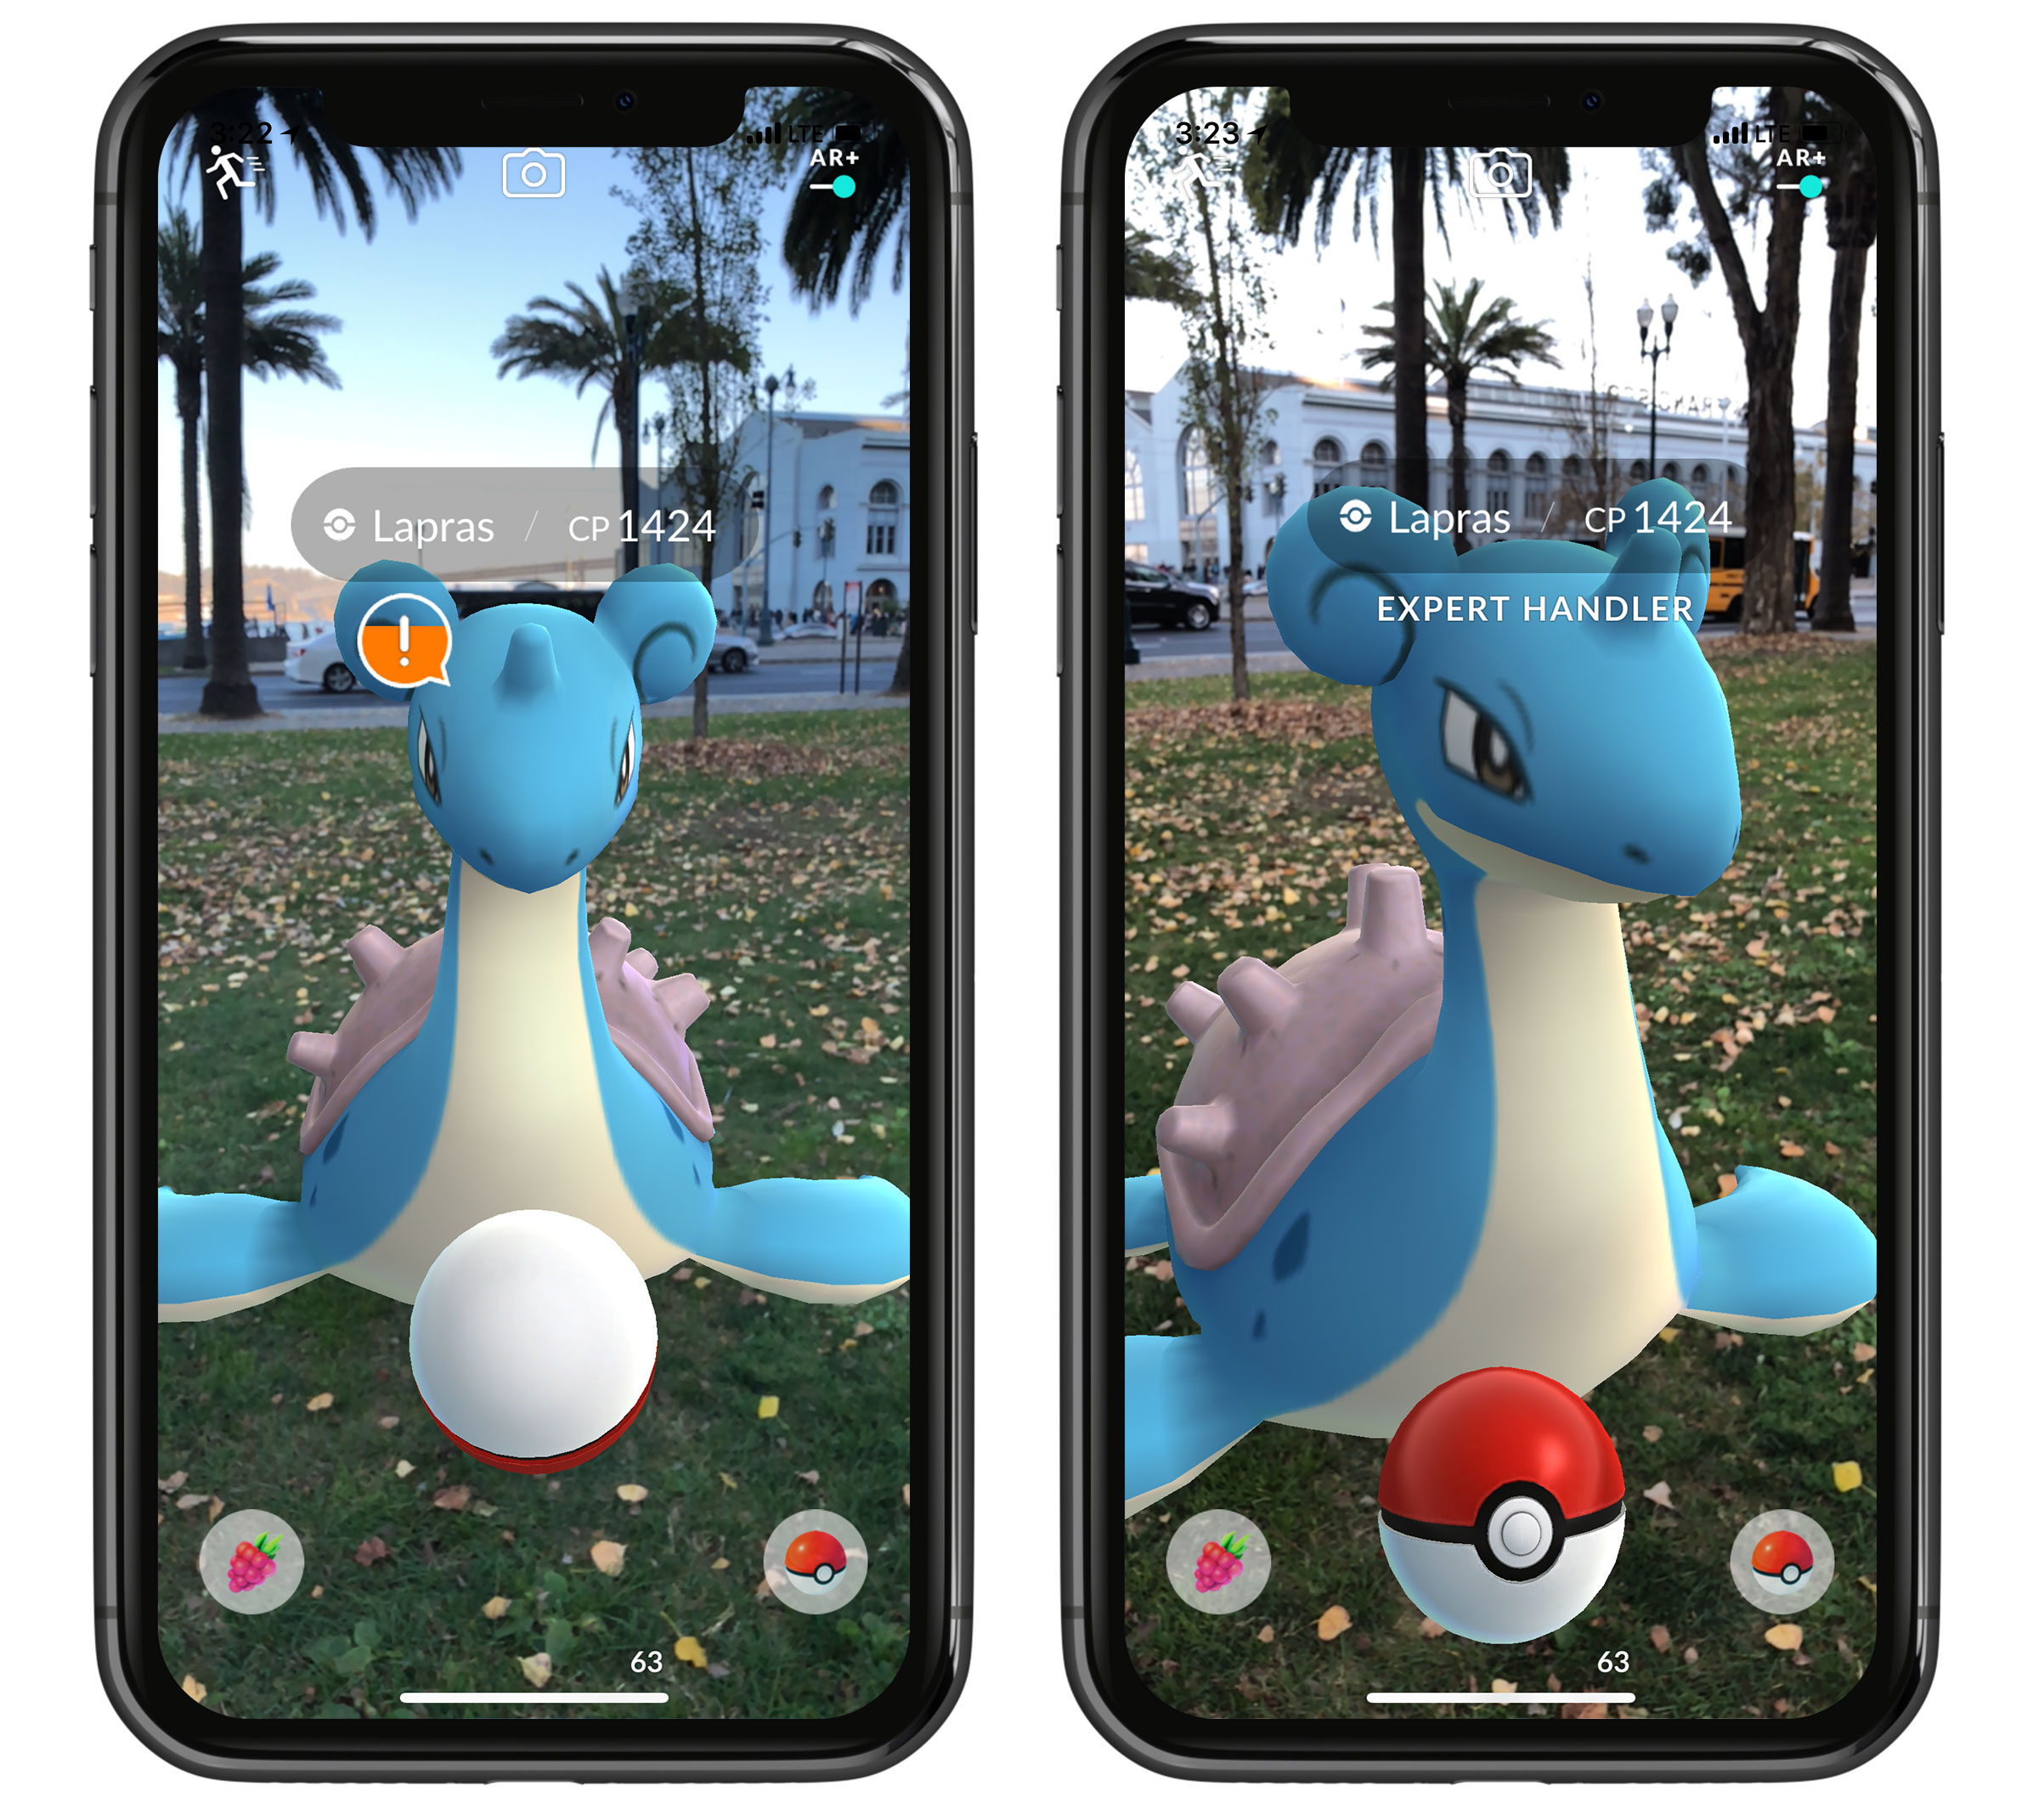
\includegraphics[width=0.45\textwidth]{images/pokemongo}
      \label{sub:STARGO}
      }
    \subfloat[Microsoft HoloLens - Vue au travers casque\protect\footnotemark]{
      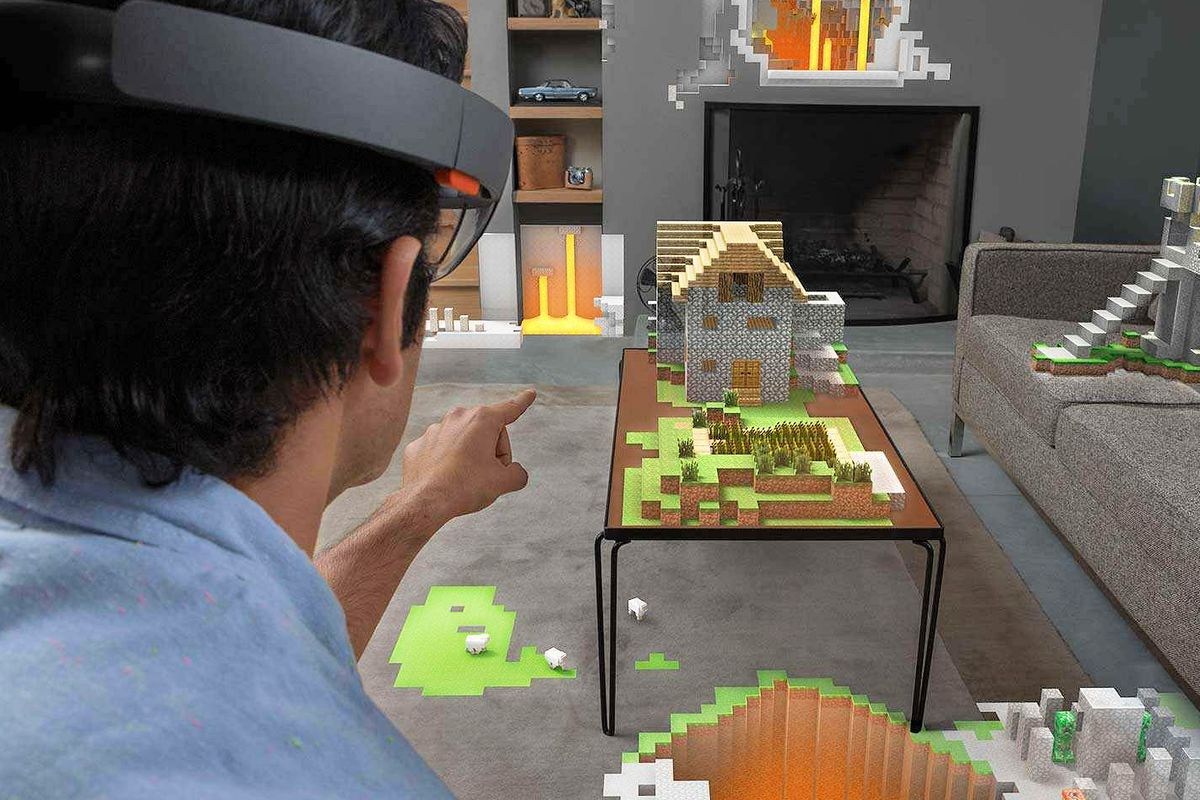
\includegraphics[width=0.45\textwidth]{images/hololens}
      \label{sub:STARHolo}
      }
\caption{Réalité augmentée vue au travers}
\label{fig:STAR}
\end{figure}
\footnotetext{Source: \href{https://pokemongolive.com/fr/}{Pokemon GO}}
\footnotetext{Source: \href{https://www.microsoft.com/fr-fr/hololens}{Microsoft HoloLens}}

\paragraph{Réalité augmentée spatiale}
% Trouver qui l'a inventé et quand
La réalité augmentée spatiale, plus communément appelé \emph{Spatial Augmented Reality (SAR)} est une technique de visualisation de la réalité augmentée se basant sur un dispositif de projection. Les éléments virtuels qui viennent "augmenter" le monde réel sont alors projetés dans l'espace (fig~\ref{fig:SAR}), d'où le terme spatiale. Cette notion d'augmentation de l'espace tend à rendre cette technologie naturellement collaborative car les projections ne dépendent pas d'un dispositif visuel personnel et sont obligatoirement partagées. La SAR permet aussi de favoriser le développement d'interface tangible, en effet, la visualisation se faisant directement sur les objets physiques, la tendance à développer des interfaces en communion avec ceux ci est très forte car très naturel.

\begin{figure}[H]
\centering
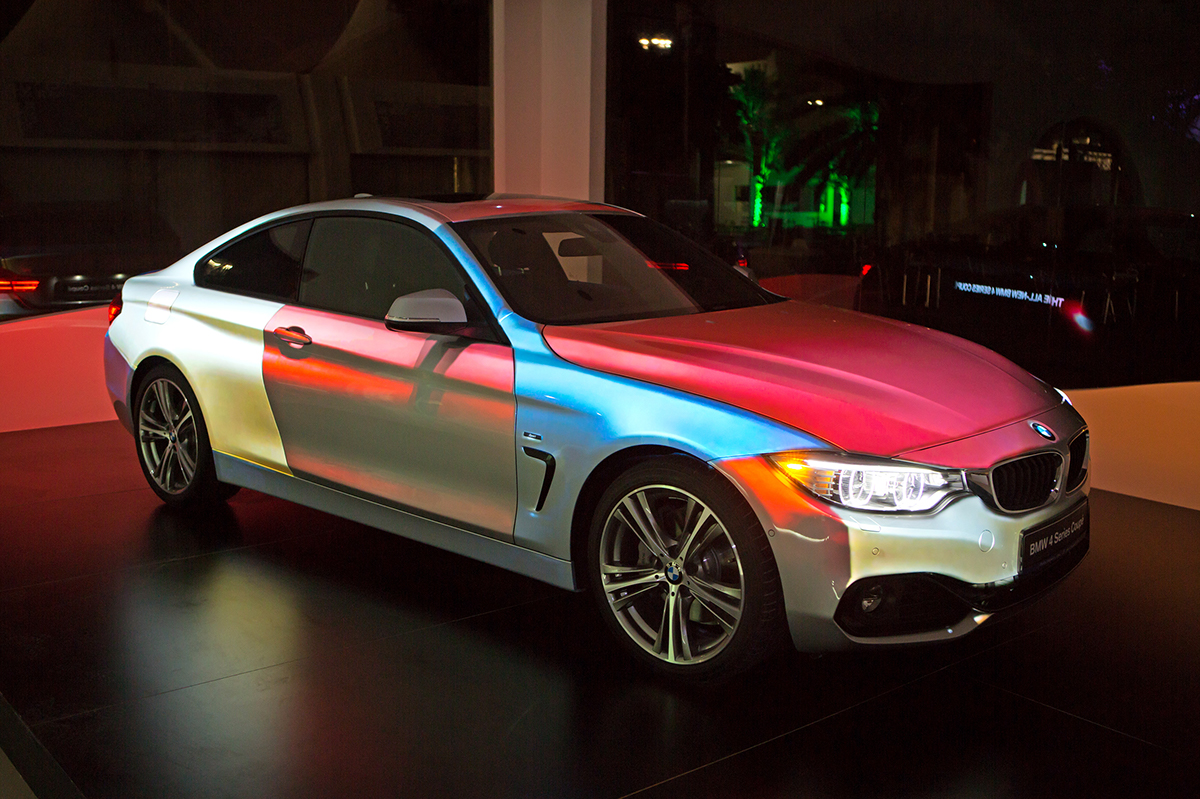
\includegraphics[width=0.5\textwidth]{images/SARMappingCar2}
\caption{Présentation d'une voiture en utilisant de la réalité augmentée spatiale\protect\footnotemark}
\label{fig:SAR}
\end{figure}
\footnotetext{Source: {Google Image}}

\paragraph{Interface tangible}
Une interface utilisateur tangible ou \emph{Tangible User Interface (TUI)} est une interface utilisateur via laquelle des objets physiques, ou encore le toucher, permettent de manipuler des données numériques (fig~\ref{sub:TUI}). Les interfaces utilisateurs tangibles remplacent très souvent les interfaces utilisateur graphiques (fig~\ref{sub:GUI}) où \emph{Graphical User Interface (GUI)} dans la plupart des application de réalité augmentée car elles fournissent un contrôle direct à l'utilisateur sur ce qu'il souhaite manipuler (par opposition au contrôle indirect, comme la souris, nécessaire à la manipulation des GUI).

\begin{figure}[H]
    \centering
	\subfloat[Interface Utilisateur Graphique (GUI)\protect\footnotemark]{
      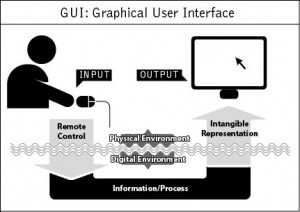
\includegraphics[width=0.45\textwidth]{images/GUI}
      \label{sub:GUI}
      }
    \subfloat[Interface Utilisateur Tangible (TUI)\protect\footnotemark]{
      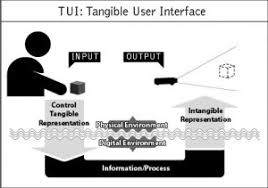
\includegraphics[width=0.45\textwidth]{images/TUI}
      \label{sub:TUI}
      }
\caption{Différences des interfaces utilisateurs}
\label{fig:GUITUI}
\end{figure}
\footnotetext{Source: \href{http://iconlibrary.iconshock.com/design/from-gui-to-tui/}{Icon Library - From GUI to TUI}}
\footnotetext{Source: \href{http://iconlibrary.iconshock.com/design/from-gui-to-tui/}{Icon Library - From GUI to TUI}}

\paragraph{Calcul haute performance}
Le calcul haute performance ou \emph{General-Purpose computing on Graphics Processing Units (GPGPU)} désigne une méthode de calcul utilisant la carte graphique (GPU) plutôt que le processeur (CPU). Cette technique permet de bénéficier de la puissance de la carte graphique afin de réaliser du calcul en parallèle et est très souvent utilisée pour la plupart des traitement lourd comme par exemple le rendu d'une scène 3D, l'encodage de vidéo, les simulations physiques (particules) etc. Cette technique repose sur le grand nombre de cœurs présent dans les cartes graphiques (contrairement aux processeurs) et sur la capacité de chacun de ces cœurs à effectué des opérations simples de manière très efficace. Le calcul haute performance ne peut cependant pas ce passer du CPU qui va être principalement utilisé pour récolter et transférer les données traités ou à traiter.
% Expliquer comment ca marche (carte graphique beaucoup de coeur pour faire des opérations simple, CPU pas beaucoup de coeur donc plus lent)
% Ajouter image comparaison

\begin{figure}[H]
\centering
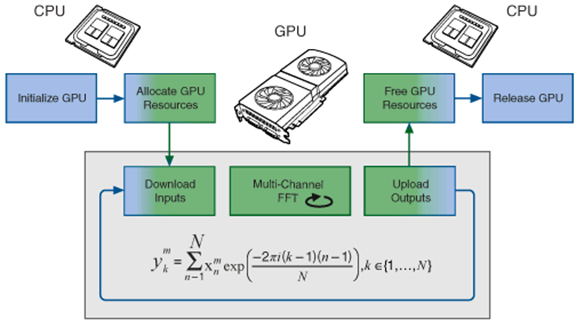
\includegraphics[scale=0.7]{images/gpuworkflow}
\caption{Exemple de calcul de la FFT sur GPU\protect\footnotemark}
\label{fig:gpgpu}
\end{figure}
\footnotetext{Source: \href{http://www.ni.com/white-paper/14077/fr/}{National Instruments}}


\chapter{État de l'art}

Intro

\section{PapARt}

\section{Système de réalité augmentée spatiale}

\section{Bilan}
 
\chapter{Analyse des besoins}

Intro

\section{Besoins fonctionnels}

Après une analyse des besoins fonctionnels du projet, nous avons défini deux sous catégories. D'un côté, les besoins [...], de l'autre, les besoins [...].

\subsection{Sous-partie 1}

Bla

\subsection{Sous-partie 2}

Bla

\newpage

\section{Besoins non-fonctionnels}

Comme précédemment, nous avons choisi de distinguer deux catégories pour les besoins non-fonctionnels. D'une part, nous avons les besoins non-fonctionnels pour les [...], et d'autre part ceux pour [...]. Nous avons aussi pris en compte les contraintes de développement, que nous détaillerons à la fin de cette partie.

\subsection{Sous-partie 1}

Bla\\

Aperçu du rendu souhaité :

\begin{figure}[!h]
\begin{center}
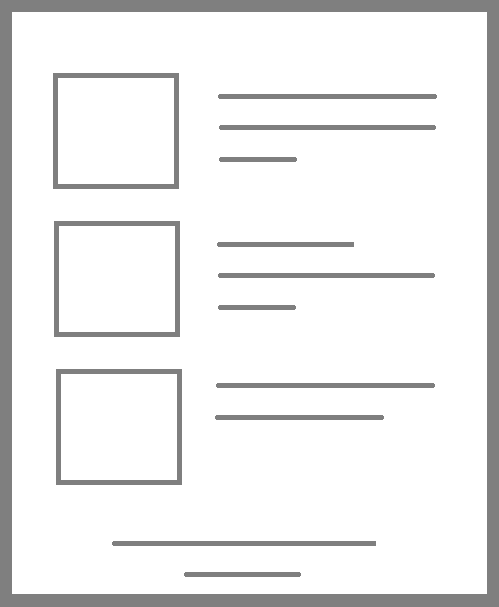
\includegraphics[height=10cm]{besoins/rendu}
\end{center}
\caption{Rendu attendu}
\end{figure}

\subsection{Sous-partie 2}

Bla

\newpage

\section{Développement}

Intro

\subsection{Tâches}

Bla\\


%tableau à taille fixée sur certaines colonnes (param sur la ligne \begin{tabularx}, voir wiki pour plus d'info sur la syntaxe
\begin{figure}[!h]
\begin{center}
\begin{tabularx}{17cm}{|c|p{6cm}|X|}
  \hline
  Priorité & Nom & Raison\\
  \hline
  1 & Tache 1 & Doit être vérifié en premier car sinon [...] \tabularnewline
  2 & Tache 2 & On doit pouvoir [...] \tabularnewline
  3 & Tache 3 & Comme les principales fonctionnalités permettant de tester sont opérationnelles, nous pouvons passer à cette tâche. \tabularnewline
  4 & Tache 4 & Parce que [...] \tabularnewline
  5 & Tache 5 & La tache 5 fait partie des principales [...]. \tabularnewline
  6 & Tache 6 & Dernière fonctionnalité essentielle à mettre en place. \tabularnewline
  7 & Tache 7 & Non-essentiel, mais apporterait un plus au projet. \tabularnewline
  8 & Tache 8 & Non-essentiel, mais apporterait un plus au projet. \tabularnewline
  \hline
\end{tabularx}
\end{center}
\caption{Tableau récapitulatif des tâches}
\end{figure}

\subsection{Tests}

Bla\\

\begin{figure}[!h]
\begin{center}
\begin{tabularx}{17cm}{|p{6cm}|X|}
  \hline
  Fonctionnalité & Test\\
  \hline
  Fonction 1 & Quand [...], vérifier [...]. \tabularnewline
  & Et quand [...], vérifier [...]. \tabularnewline
  Fonction 2 & Vérifier [...]. \tabularnewline
  Fonction 3 & Vérifier [...]. \tabularnewline
  Fonction 4 & Avoir [...]. \tabularnewline
  Fonction 5 & Accéder à [...]. \tabularnewline
   & Vérifier que [...]. \tabularnewline
  Fonction 6 & Accéder à [...]. \tabularnewline
   & Et vérifier [...]. \tabularnewline
  Fonction 7 & Installer [...]. \tabularnewline
   & Vérifier [...]. \tabularnewline
  Fonction 8 & Compter [...]. \tabularnewline
  \hline
\end{tabularx}
\end{center}
\caption{Tableau récapitulatif des tests}
\end{figure}

\chapter{Autre partie}

Dans cette partie nous cherchons à décrire dans un premier temps [...], puis, c[...].

\section{Partie 1}

Intro

\subsection{Sous-partie 1}

\begin{figure}[!ht]
\begin{center}

\includegraphics[height=12cm]{autre_partie/image1}
\end{center}
\caption[autre partie générale]{autre partie image 1\protect\footnotemark}
%\floatfoot{Source: (Citation command)}
% avec le package "floatrow"
\end{figure}

%footnote protected pour apparaitre dans la légende d'une image
\footnotetext{Schéma d'après : \textit{Auteur 1 \& Propriétaire image}, LICENCE (cf. ref. \cite{cite4})}

\newpage{}

\subsection{Sous-partie 2}

\begin{figure}[!ht]
\begin{center}

\includegraphics[height=12cm]{autre_partie/image2}
\end{center}
\caption[autre partie]{autre partie globale de notre quelque chose}
\end{figure}

Nous retrouvons ici, blabla\footnote{Application bla - Interface blabla} [...].

\subsubsection{Sous-sous-partie 1}

Le bla (cf. ref. \cite{cite6}) est [...]:

\begin{itemize}
\item item1;
\item item2;
\item item3;
\item item4;
\item item5.
\end{itemize}

\newpage

\subsubsection{Sous-sous-partie 2}

%Les lignes :
% \setcounter{secnumdepth}{4}
% \setcounter{tocdepth}{4}
%dans le fichier "main.tex" permettent de faire en sorte que les paragraphes soient interprété comme des titres de niveau 5
\paragraph{Paragraphe 1 (agissant comme titre niveau 5)}
%forcer un saut de ligne
~\\
\hskip7mm

\begin{figure}[!ht]
\begin{center}

\includegraphics[height=6cm]{autre_partie/image3}
\end{center}
\caption[Structure d'unz autre chose]{Structure d'une autre chose\protect\footnotemark}
\end{figure}

Ce schéma représente bla.

\footnotetext{Schéma et explication d'après le wiki bla (cf. ref. \cite{cite0})}

\paragraph{Paragraphe 2}
~\\
\hskip7mm

%fixer les floats précédemment définis
%\FloatBarrier

Bla

\subparagraph{Sous-paragraphe 1}
~\\
\hskip7mm

Bla

\begin{figure}[H]
\begin{center}

\includegraphics[height=10cm]{autre_partie/image4}
\end{center}
\caption{Diagramme de truc}
\end{figure}

\subparagraph{Sous-paragraphe 2}
~\\
\hskip7mm

Bla\\

Bla

\subparagraph{Sous-paragraphe 3}
~\\
\hskip7mm

Bla

\subsubsection{Sous-sous-partie 3}

Bla

\section{Partie 2}

Bla

\footnotetext{D'après le schéma disponible sur la documentfation officielle disponible sur le site blalbla}

Bla

\subsection{Sous-partie 1}

Bla

\subsection{Sous-partie 2}

Bla

\paragraph*{Paragraphe 1 (n'apparaitra pas dans l'index)}
Bla

\paragraph*{Paragraphe 2}
Bla

\paragraph*{Paragraphe 3}
Bla

\subsection{Sous-partie 3}

Bla

\chapter{Résultats}

\section{Partie 1}

Intro

\subsection{Sous-partie 1}

\paragraph*{Paragraphe 1 (n'apparaitra pas dans l'index)} Bla

\paragraph*{Paragraphe 2} Bla

\paragraph*{Paragraphe 3} Bla

\subsection{Sous-partie 2}

Bla

\subsection{Sous-partie 3}

Bla

\section{Partie 2}

Intro

\subsection*{Sous-partie 1 ('apparaitra pas dans l'index)} Bla

\paragraph*{Paragraphe 1 ('apparaitra pas dans l'index)} Bla

\paragraph*{Paragraphe 2} Bla

\paragraph*{Paragraphe 3} Bla

\newpage

\subsection*{Sous-partie 2}

Bla

%galerie d'image
\begin{figure}[htp]
  \centering
  \subfloat[Première image]{\label{fig:première}
\includegraphics[scale=0.8]{resultats/gallerie}}
  ~ %espace entre deux images sur une même ligne
  \subfloat[Deuxième image]{\label{fig:deuxième}
\includegraphics[scale=0.8]{resultats/gallerie}}
  ~
  \subfloat[Troisième image]{\label{fig:troisième}
\includegraphics[scale=0.8]{resultats/gallerie}}
  ~\\ %saute une ligne dans la galerie d'image
  \subfloat[Quatrième image]{\label{fig:quatrième}
\includegraphics[scale=0.8]{resultats/gallerie}}
  ~
  \subfloat[Cinquième image]{\label{fig:cinquième}
\includegraphics[scale=0.8]{resultats/gallerie}}
  \caption{Différents screenshots quelque chose, en gallerie}
  \label{fig:gallerie1}
\end{figure}

\chapter{Bilan}

%Rappel du context
Intro / Rappel Contexte

Nous avons donc pu en tirer la problématique suivante :

\begin{center}
\hskip7mm
Problématique du sujet
\end{center}

Bla

Bla\\

Bla\\

%Rappel des résultats
Bla

Bla\\

Bla

Bla

\newpage

%Conclusion/Perspectives
Bla

Bla\\

Bla

%Ne pas numéroter cette partie
\part*{Annexes}
%Rajouter la ligne "Annexes" dans le sommaire
\addcontentsline{toc}{part}{Annexes}

\chapter*{Annexe 1}
\addcontentsline{toc}{chapter}{Annexe 1}

%changer le format des sections, subsections pour apparaittre sans le num de chapitre
\makeatletter
\renewcommand{\thesection}{\@arabic\c@section}
\makeatother

%recommencer la numérotation des section à "1"
\setcounter{section}{0}

Intro

\section{Partie 1}

Bla

\subsection{Sous-partie 1}

Bla

\subsection{Sous-partie 2}

Bla

\subsection{Sous-partie 3}

Bla

\section{Partie 2}

Bla

\subsection{Sous-partie 1}

Bla

\subsection{Sous-partie 2}

Bla

\subsection{Sous-partie 3}

Bla

\chapter*{Annexe 2}
\addcontentsline{toc}{chapter}{Annexe 2}

%recommencer la numérotation des section à "1"
\setcounter{section}{0}

Intro

\section*{Prérequis}
\addcontentsline{toc}{section}{Prérequis}

Bla

\begin{itemize}
\item item1;
\item item2;
\item item3;
\item item4.
\end{itemize}

Bla

\section{Partie 1}

Bla

\subsection{Sous-parie 1}

Bla

\subsection{Sous-parie 2}

Bla

\section{Partie 2}

\begin{center}
\textsc{Attention !}

\textit{Texte d'avertissement}
\end{center}

Bla

\newpage

\section{Partie 3}

Bla

\begin{figure}[!ht]
\begin{center}
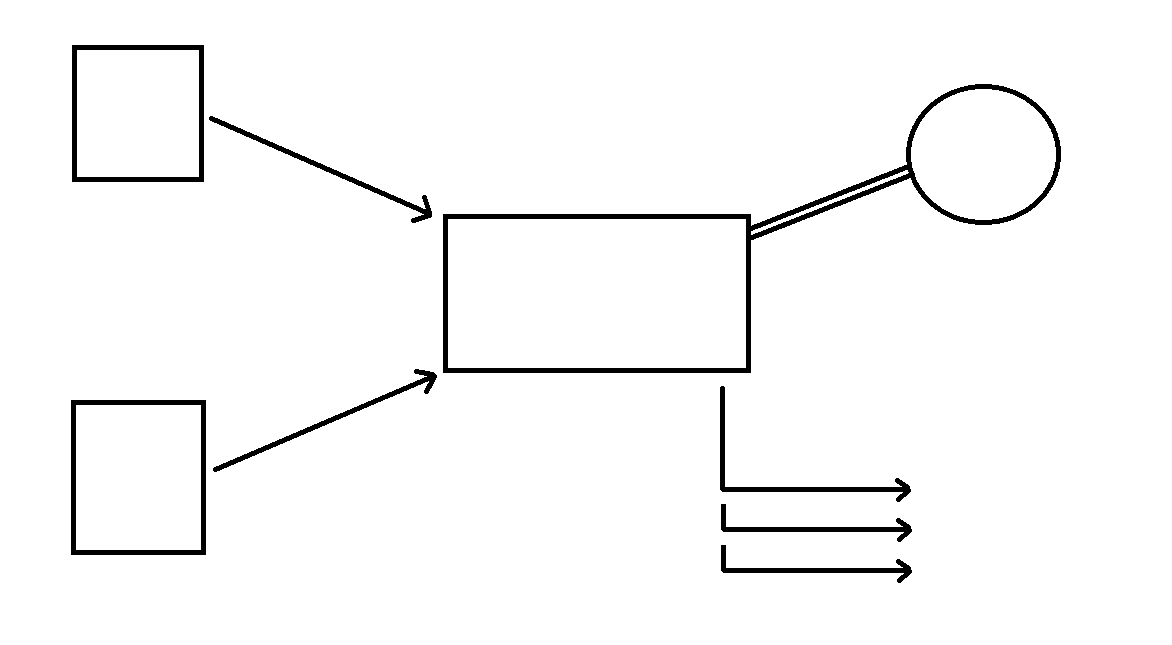
\includegraphics[height=8cm]{presentation/schema}
\end{center}
\caption[schema]{Presentation schema}
\end{figure}

\paragraph*{Paragraphe 1}
~\\
\hskip7mm

Bla

\paragraph*{Paragraphe 2}
~\\
\hskip7mm

Bla

\paragraph*{Paragraphe 3}
~\\
\hskip7mm

Bla

\chapter*{Annexe 3 - Unity diagramme d'exécution des fonctions}
\addcontentsline{toc}{chapter}{Annexe 3 - Unity diagramme d'exécution des fonctions}
\label{annexe:unity}

\begin{figure}
\centering
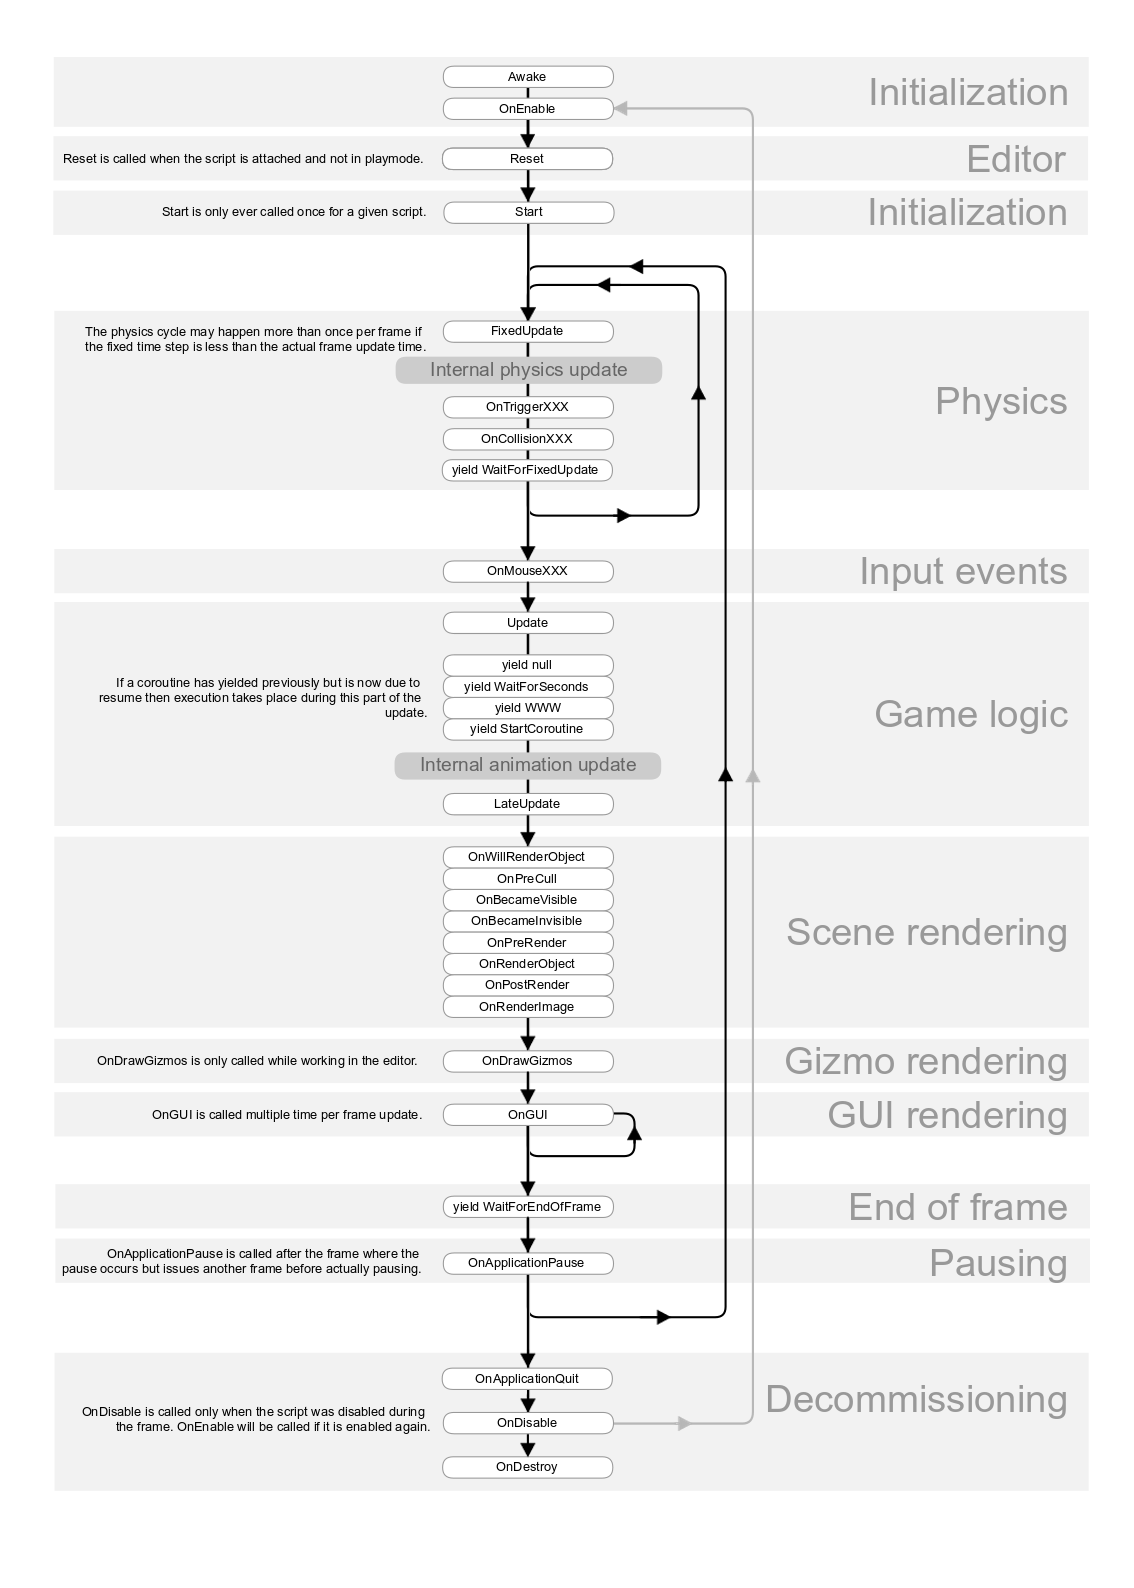
\includegraphics[width=\linewidth]{images/monobehaviour_flowchart}
\end{figure}

\newpage

%récupérer les citation avec "/footnotemark"
\nocite{*}

%choix du style de la biblio
\bibliographystyle{plain}
%inclusion de la biblio
\bibliography{bibliographie.bib}
%voir wiki pour plus d'information sur la syntaxe des entrées d'une bibliographie

\end{document}